\graphicspath{{./images/}}

\chapter{Bausteinsicht}

\section{Beschreibung}

Die Architektur für die Applikation wird mittels Schichten realisiert. Die Präsentationsschicht ist auf dem WebServer während sich die anderen vier auf dem Onboarding Server befinden. Die einzelnen Komponenten wurden gruppiert um die Übersicht zu wahren. Auf der nächsttieferen Ebene sind diese Komponenten detaillierter aufgeführt.

\newgeometry{left=2.5cm, right=2.5cm, bottom=2.5cm, top=2.5cm}
\begin{landscape}
\section{Ebene 1 : Layer Architektur}

\begin{figure}[H]
	\centering
	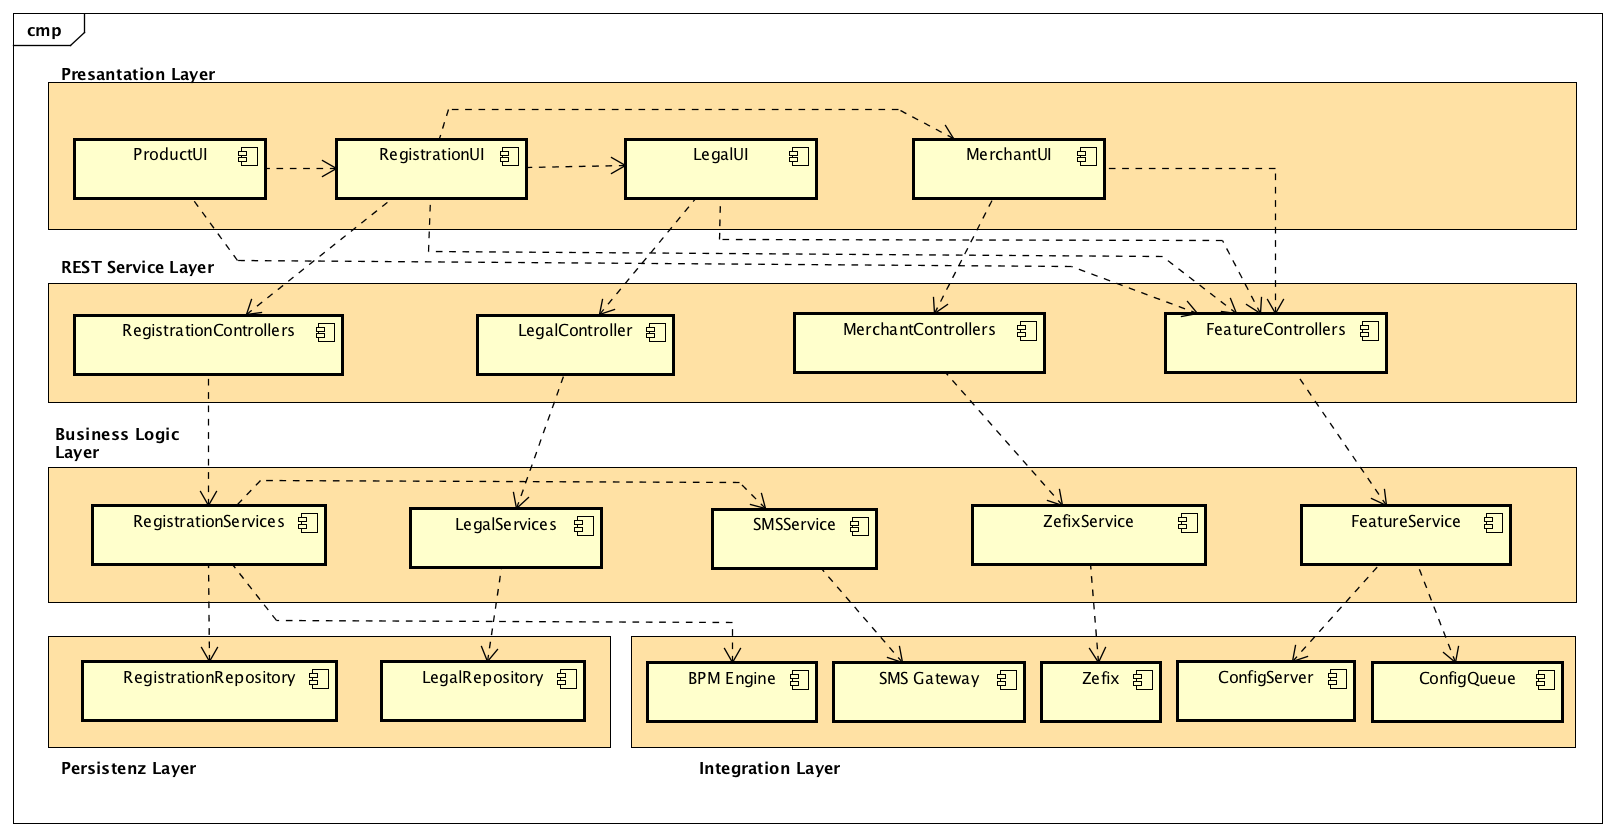
\includegraphics[scale=0.6]{ComponentLevel1.png}
	\caption{Bausteinsicht Ebene 1}
\end{figure}

\end{landscape}
\restoregeometry

\begin{table}[H]
	\centering
	\caption{Presentation Layer}
	\begin{tabular}{ | p{4.5cm} | p{10.5cm} | }
		\toprule
		{\textbf{Komponente}} & {\textbf{Beschreibung}} \\
		\midrule
		ProductUI &  Stellt die einzelnen Produktoptionen von TWINT dar welche der Benutzer auswählen kann.\\ \hline
		RegistrationUI  &  Beinhaltet die Felder für den Start des Registrierungsprozesses sowie für die \textit{\gls{MTAN}} Verifikation.\\ \hline
		LegalUI &  Zeigt rechtliche Dokumente wie Allgemeine Geschäftsbedienungen an.\\ \hline
		MerchantUI & Enthält das Formular für die Koordinaten des Händler nach der erfolgreichen Verifikation des \textit{\gls{MTAN}} Codes und ist für den Abschluss der Registration zuständig.\\
		\bottomrule
	\end{tabular}
\end{table}

\begin{table}[H]
	\centering
	\caption{REST Service Layer}
	\begin{tabular}{ | p{4.5cm} | p{10.5cm} | }
		\toprule
		{\textbf{Komponente}} & {\textbf{Beschreibung}} \\
		\midrule
		RegistrationControllers &  Schnittstelle für den Registrierungsprozess. Startet den Prozess und führt die Verifikation des \textit{\gls{MTAN}} Codes durch.\\ \hline
		LegalController &  Schnittstelle welche rechtliche Dokumente liefert. \\ \hline
		ExternalServiceController &  Schnittstelle zu externen Diensten. \\ \hline
		FeatureControllers & Schnittstelle für das Abfragen der aktiven Features. \\
		\bottomrule
	\end{tabular}
\end{table}

\begin{table}[H]
	\centering
	\caption{Business Logic Layer}
	\begin{tabular}{ | p{4.5cm} | p{10.5cm} | }
		\toprule
		{\textbf{Komponente}} & {\textbf{Beschreibung}} \\
		\midrule
		RegistrationService &  Enthält sämtliche Logik für die Aufbereitung der Registrierungsanfrage an die Workflow Engine. Führt die Verifikation des \textit{\gls{MTAN}} Codes durch welcher via SMS versendet Wurde.\\ \hline
		LegalService &  Stellt die Dienste für das Abfragen den rechtlichen Dokumente bereit. \\ \hline
		FeatureService &  Verwaltet die aktuell eingeschalteten Features welche aktiviert sind. Holt sich die neuen Konfigurationen automatisch nach einer Benachrichtigung durch die Message Queue. \\ \hline
		ExternalServices & Schnittstelle zu diversen externen WebServices der Post, des Schweizer Bundes und des Handelsregister. \\
		\bottomrule
	\end{tabular}
\end{table}

\begin{table}[H]
	\centering
	\caption{Persistenz Layer}
	\begin{tabular}{ | p{4.5cm} | p{10.5cm} | }
		\toprule
		{\textbf{Komponente}} & {\textbf{Beschreibung}} \\
		\midrule
		RegistrationRepository &  Speichert die Registrierungsdaten, den \textit{\gls{MTAN}} Code sowie die Requests, welche nicht direkt zur Workflow Engine gesendet werden können. \\ \hline
		LegalRepository &  Holt die rechtlichen Dokumente aus dem Datenspeicher. \\
		\bottomrule
	\end{tabular}
\end{table}

\begin{table}[H]
	\centering
	\caption{Integration Layer}
	\begin{tabular}{ | p{4.5cm} | p{10.5cm} | }
		\toprule
		{\textbf{Komponente}} & {\textbf{Beschreibung}} \\
		\midrule
		3rd Party Service &  Schnittstelle zu externen Diensten der Post und des Handelsregisters\\ \hline
		ConfigService &  Dienste für die Konfiguration.\\ \hline
		Internal Service &  Interne Dienste wie SMS Gateway und Mailserver\\ \hline
		BPM Engine & Verarbeitet die Registrierungsdaten im hinterlegten Workflow, beschrieben in Kapitel \ref{businesscase}\\
		\bottomrule
	\end{tabular}
\end{table}
\newpage


\section{Ebene 2 : RegistrationUI}
Anhand des Registrierungsintefaces soll der generelle Aufbau illustriert werden. Sämtliche UI Teile besitzen eine View in Form eines HTML Files. Der Controller steuert die Interaktion des Benutzers und sendet die Daten via Services an den \textit{\gls{REST}} Controller auf dem Server. Der FeatureService enthält Methoden um zu Prüfen ob einzelne Features im Interface aktiv sind oder nicht. Siehe dazu auch Kapitel \ref{toggles} Feature Toogles.

\begin{figure}[H]
	\centering
	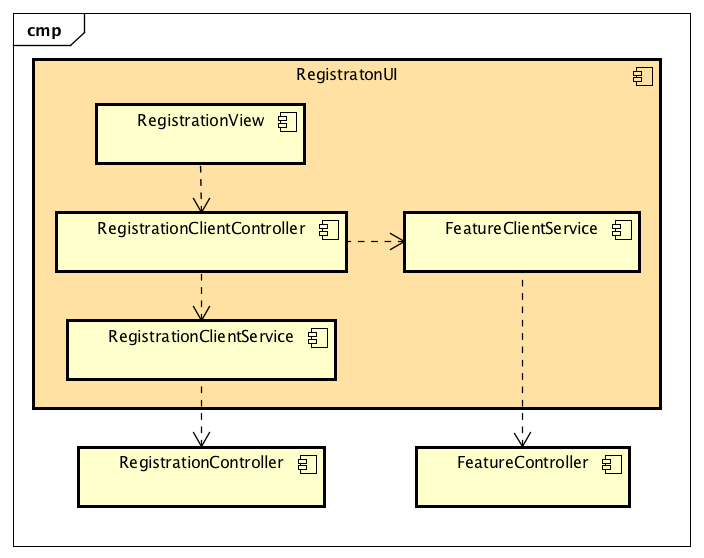
\includegraphics[scale=0.8]{WebComponentLevel2.png}
	\caption{Registrations Web Interface Ebene 2}
\end{figure}
\newpage
\section{Ebene 2 : RegistrationServices}
\label{reg-service}

Der Registrierungsservice kümmert sich um die Aufbereitung der Daten für die Workflow Engine sowie die Übertragung der Daten. Er verwendet den SMS- und dem MailService um Nachrichten an den Händler zu schicken. Nach der Bestätigung des Benutzers, durch den \textit{\gls{MTAN}} Code, speichert er die Daten in der Datenbank. Der SchedulerService prüft regelmässig, ob neue Registierungen pendent sind, und sendet sie an die \textit{\gls{BPM}} Engine. Sollte bei der Kommunikation ein Fehler auftreten, wird zu einem späteren Zeitpunkt nochmals versucht die Daten an den Workflow zu schicken. {\color{red} Wie lange geht das ?}
\begin{figure}[H]
	\centering
	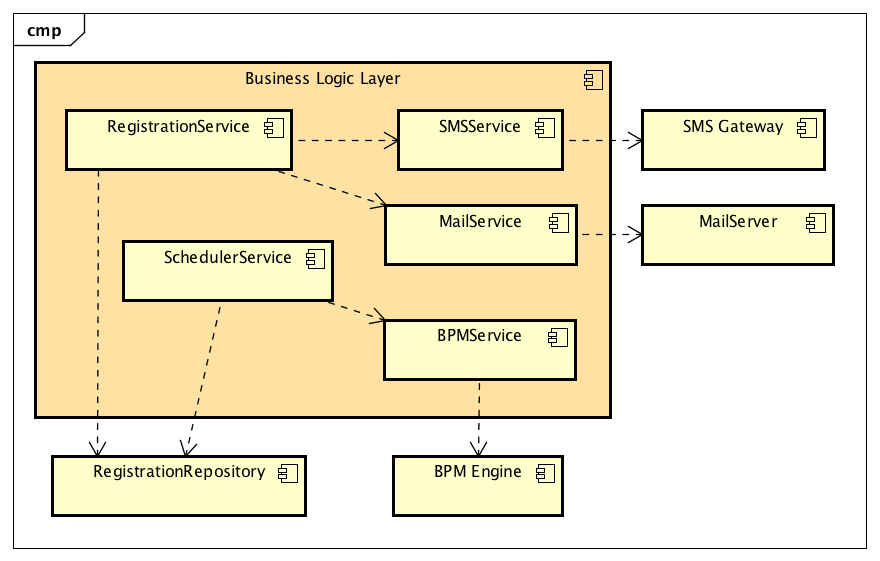
\includegraphics[scale=0.65]{RegistrationServicesLevel2.png}
	\caption{Registrations Services Ebene 2}
\end{figure}
\newpage
\section{Ebene 2 : ExternalServices}

Die ExternalServices bestehen aus den Diensten für die Unternehmensindentifikation, Handelsregisterauszug und Adressüberprüfungen. Sie erlauben eine vereinfachte Registrierung des Händler welcher dadurch nicht alle Daten selber eingeben respektive zusammensuchen muss.

\begin{figure}[H]
	\centering
	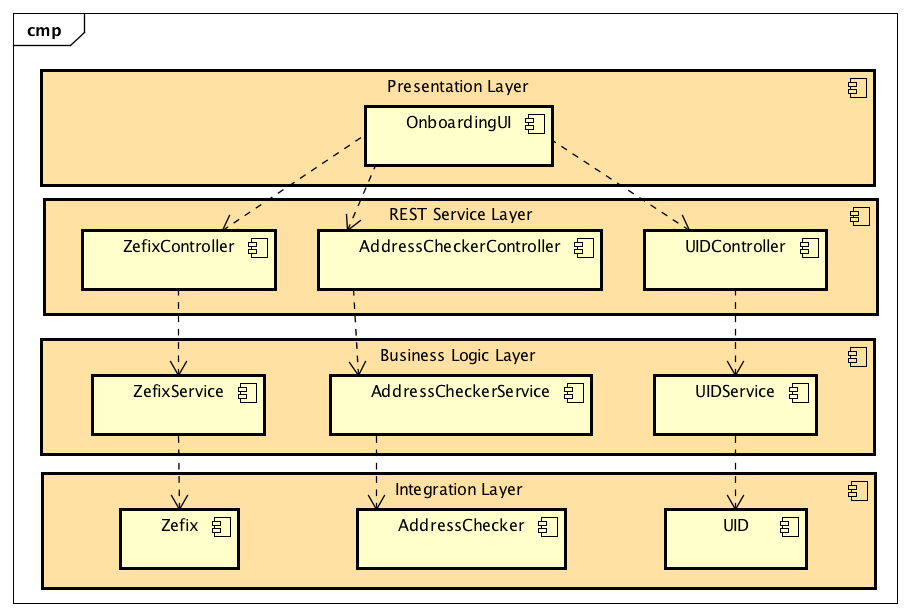
\includegraphics[scale=0.65]{ExternalServicesLevel2.png}
	\caption{Externe Services Ebene 2}
\end{figure}